\section{Druhá mechanická varianta}


Druhá mechanická varianta má oproti první verzi daleko vetší počet možných kombinací.
Ovládá se pěti koly, z nichž čtyři zajišťují heslo a páté otáčí s rotační západkou, které drží dveře na svém místě.
Tato varianta taky přichází z možností dveře úplně oddělit od skříně trezoru. To by při využití jako trezor, který
má za úkol jen ochraňovat svůj obsah, sice nepřinášelo žádný velký užitek, ale při mém využití, spíše jako herní 
prvek než trezor, to může být užitečné.

\begin{figure}[htbp]
    \centering
    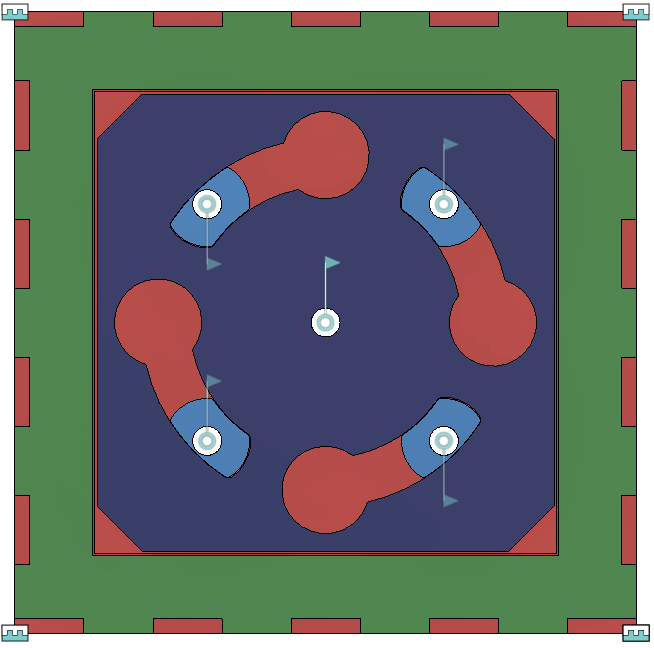
\includegraphics[width=150pt]{kapitoly/obrazky/M2/mechanizmus_odemcen.png}
    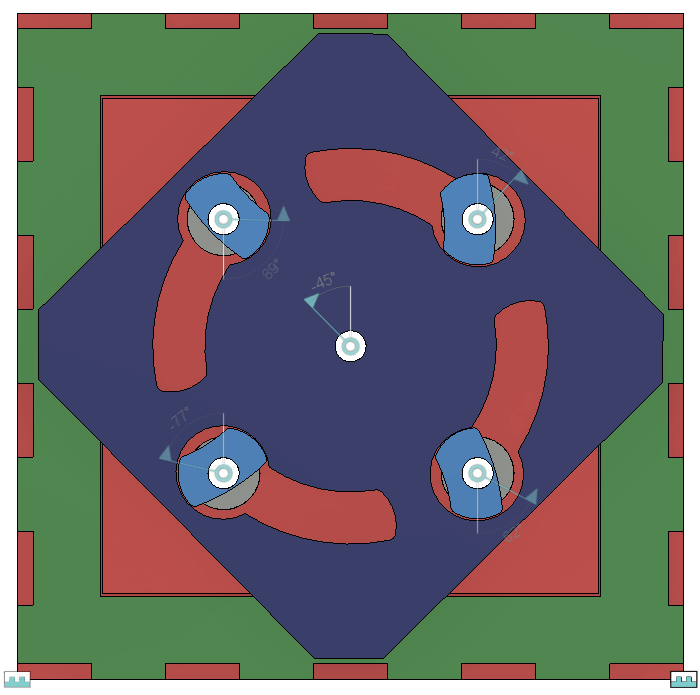
\includegraphics[width=150pt]{kapitoly/obrazky/M2/mechanizmus_zamceno.png}
    \caption{zamykací mechanizmus varianty M2}
    \label{fig:M2-mechanizmus}
\end{figure}

\begin{figure}[htbp]
    \centering
    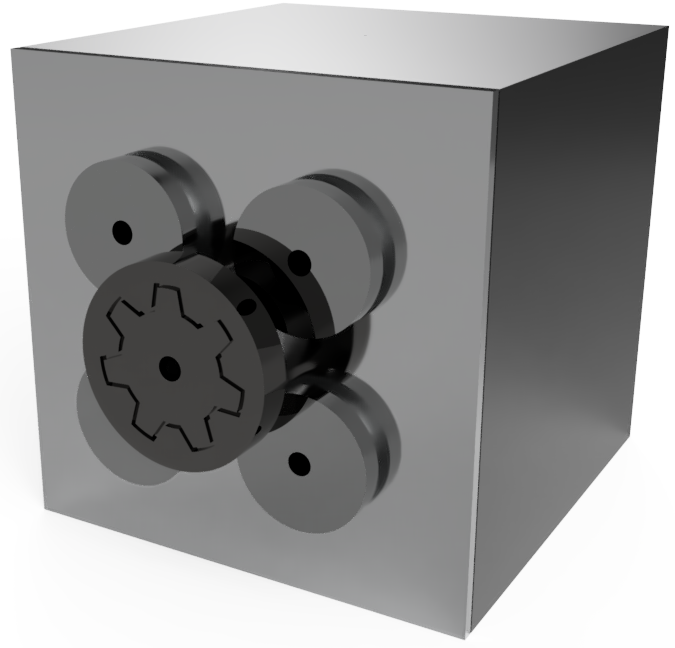
\includegraphics[width=\textwidth]{kapitoly/obrazky/M2/predni_render.PNG}
    \caption{render varianty M2}
    \label{fig:M1.0}
\end{figure}


\newpage